
\chapter{Astronomy and Epic Chronology\index{Chronology}}\label{chapter2}

\Authorline{-- Nilesh Nilkanth Oak$^{\ast}$}\footnotetext{*pp.~\pageref{chapter2}\enginline{--}\pageref{chapter2-end}. In: Kannan, K. S. and Meera, H. R. (Ed.s) (2021), \textit{Chronology and Causation: Negating Neo-Orientalism Chennai: Infinity Foundation India.}}

\lhead[{\small\thepage}\quad\small Nilesh Nilkanth Oak]{}

\begin{flushright}
\textit{(nileshoak@gmail.com)}
\end{flushright}


\section*{Pollock’s Claim for the Chronology \hfill\break of \textit{Mahābhārata} and \textit{Rāmāyaṇa} }\index{Mahabharata@\textit{Mahābhārata}}\index{Ramayana@\textit{Rāmāyaṇa}}

On the chronology of the \textit{Mahābhārata}, Pollock\index{Pollock, Sheldon} writes:

\begin{myquote}
Everything about the \textit{Mahābhārata}, from its history as a text to the history of its impact on South Asian culture, is huge and complex. \textbf{There is little hard evidence about the origins of the work} in its monumental form (eighteen books, and something on the order of a hundred thousand verses according to its own calculation). Even a cursory analysis of the manuscript data available in the critical edition reveals that the majority of the books were transmitted not orally but in reasonably stable form based on written archetypes.\textbf{ These cannot have come into being much before the beginning of the Common Era and are very likely of a much later date}. 

~\hfill (Pollock 2006a: 224) (\textit{emphasis ours})
\end{myquote}

On the chronology of the \textit{Rāmāyaṇa}, Pollock writes:

\begin{myquote}
“No convincing evidence has been offered for a pre-Ashokan date of the \textit{Rāmāyaṇa} in its monumental form (the common denominator of all our manuscripts), let alone a date before the Buddha\index{Buddha, the} (c. 400 B.C.E.). The attributions of individual verses, or whole \textit{kāvya}s,\index{kavya@\textit{kāvya}} to “Pāṇini,”\index{Panini@Pāṇini} whose own date is largely conjectural (convention puts him in the mid-fourth century B.C.E.), are late and without a shred of reliability.” 

~\hfill (Pollock 2006a: 81)
\end{myquote}

In effect, he considers timing of 200 BCE through 400 CE for the first text of \textit{Mahābhārata}\index{Mahabharata@\textit{Mahābhārata}} and about 150 BCE for the first text of \textit{Rāmāyaṇa}.\index{Ramayana@\textit{Rāmāyaṇa}}


\section*{How does Pollock Arrive at his Chronology Claims?}

His claim for the above chronology\index{Chronology} of the \textit{Mahābhārata} and the \textit{Rāmāyaṇa}, is based on pleading for his claims, in a circular fashion, by alluding to absence of evidence for existence of manuscripts or inscriptions, prior to his claimed time (200 BCE through 400 CE), for the writing of these epics.

Pollock’s\index{Pollock, Sheldon} entire approach to chronology, not just the chronology of the \textit{Mahābhārata} and the \textit{Rāmāyaṇa} but also any instance of ancient Indian chronology, is through a confusing combination of ‘irrelevancies’, absence of evidence coupled with alleged consensus of Indologists, in turn supported by lack of evidence.

Here are a few illustrations of how Pollock arrives at his claims for the timing of various things Indian and how he connects them, without any logical relevance, to his claims for the dating of Indian epics.

\subsection*{1. Irrelevancies; \hfill\break Absence of Evidence = Evidence of Absence}

Pollock writes:

\begin{myquote}
“Patañjali\index{Patanjali@Patañjali} … appears to have lived at a moment of transition in intellectual history when the tradition of systematic study of grammar had somehow been disrupted…Patañjali goes on to cite a number of Vedic passages that identify additional functions of grammatical knowledge. These include the ability to distinguish between those who employ correct language forms and the “antigods” (\textit{asura}) with their deviant usage; avoiding the potentially fatal consequences of the improper use of a word; acquisition of true learning, which consists in understanding and not just reproducing...” 

~\hfill (Pollock 2006a: 46-47)
\end{myquote}

And in what way Pollock considers this relevant for the dating of the \textit{Mahābhārata}? This is never clear. Even more confusing, although irrelevant, is how Pollock goes on to investigate the date of Patañjali:

\begin{myquote}
“The problem here is not the data but the date of the \textit{Mahābhāṣya}\index{Mahabhasya@\textit{Mahābhāṣya}} itself. The evidence usually adduced for placing Patañjali\index{Patanjali@Patañjali} around 150 B.C.E. is subject to a number of uncertainties, not least the possibility that the grammarian might have been citing predecessors in the passages taken as grounds for early dating. \textbf{Arguments placing him as late as the middle of the second century C.E. are entirely credible.”} 

~\hfill (Pollock 2006a:80) (\textit{emphasis ours})
\end{myquote}

And what is the logical connection between this claim for the ‘credible arguments for Patañjali in second century CE’ and the chronology\index{Chronology} of the \textit{Mahābhārata}?\index{Mahabharata@\textit{Mahābhārata}} Pollock\index{Pollock, Sheldon} continues with additional irrelevancies:

\begin{myquote}
“Patañjali refers only once to a poet by name, \textit{vārarucaṁ kāvyam}\index{kavya@\textit{kāvya}} (on 4.3.101, which is also his sole use of the word \textit{kāvya} in the sense of literature), and he refers to only three literary works (\textit{ākhyāyikā}s, on 4.2.60). Since the grammarian could be citing older grammatical materials (even as he elsewhere cites older philosophical materials) in two key historical passages… Frauwallner\index{Frauwallner, Erich} argues for a mid-second-century C.E. date (1960, especially pp. 111ff.); so Sircar 1939a. If the \textit{Mahābhāṣya} is taken as a composite work (denied by Cardona 1978), any precise dating of course becomes impossible. At all events, Patañjali’s is hardly “the only really firm initial date known in Sanskrit writing”(Zvelebil 1992:102).” 

~\hfill (Pollock 2006a: 80-81ff)
\end{myquote}

Pollock does not tell us how many counts of referrals to poets by name, or how many counts of literary works would have been sufficient to question the credibility of the claim for Patañjali in 2nd century CE. He does not tell us the logic employed by Frauwallner. Why did Pollock bother to refer to all this speculation if any precise dating was considered impossible ‘if ‘\textit{Mahābhāṣya}’ is treated as a composite work’, which he seems to suggest? Pollock concludes by stating that much alternate evidence exist and one need not depend on the dating of Patañjali. Of course, he nowhere states what those other ‘really firm initial dates known in Sanskrit writing’ are.


\subsection*{2. Assumed Consensus of Indologist Opinions \hfill\break and Negative Evidence}

Here is an illustration of Pollock combining ‘scholarly consensus’ with ‘negative evidence’:

\begin{myquote}
One factor in determining the beginnings of Sanskrit \textit{kāvya}\index{kavya@\textit{kāvya}} that has been mentioned so far only in passing needs detailed consideration: the place of writing in the constitution of this cultural form and the date of the invention of writing itself in India. We have seen that a new scholarly consensus places the latter at the Maurya chancery around 260 B.C.E. (chapter 1.2). Whether or not this consensus is true in all particulars, nothing suggests a date for Indic writing before that period, and much evidence from after that date serves to sustain the consensus. 

~\hfill (Pollock\index{Pollock, Sheldon} 2006a: 81-82)
\end{myquote}

\vspace{-.3cm}

\subsection*{3. Mixing of ‘Bad’ Inferences with the ‘Good’ Inferences}

Pollock often mixes ‘bad’ inference with ‘good’ inference to push his ‘bad’ claim as credible:

\begin{myquote}
“Chapter 2 sets out the grounds for thinking of Sanskrit \textit{kāvya}—a category, as noted earlier, that was clear and distinct in premodern South Asia—as a new phenomenon in Indian cultural history when it first appeared a little before the beginning of the Common Era. From the first, \textit{kāvya} was almost certainly composed and circulated (though not typically experienced) in writing;…” 

~\hfill (Pollock 2006a: 13)
\end{myquote}

\vspace{-.3cm}

\subsection*{4. Absence of Evidence as ‘Clinching’ Evidence}

Finally, an example of Pollock treating ‘absence of evidence’ as clinching evidence for his desired conclusion:

\begin{myquote}
Inscriptions, \textit{testimonia}, citations in literature, philology, the history of literary theory—every piece of evidence hard and soft thus requires locating the origins of \textit{kāvya} in the very last centuries B.C.E., perhaps as much as a millennium after the Sanskrit language is believed to have first appeared in the subcontinent. 

~\hfill (Pollock 2006a: 81)
\end{myquote}

Faulty assumptions, however unstated, of AIT\index{Aryan Invasion Theory} timeline (1500 BCE as time of “Aryan arrival”) abound.


\subsection*{Pollock’s Three Step Method}

While Pollock uses arbitrary or selective evidence and interprets it in an irrational fashion, a general pathway of his methodology can be described as follows:

Step 1: An initial hypothesis, with selectively picked (and most cases, wrongly interpreted) data which is woven into a theory

Step 2: A lot of subsequent work is produced to support this flimsy theory by usage of mutually referencing data which in turn is based on other equally flimsy theories (circular reasoning). Voluminous works are generated. This is very important in this phase. These works should support the narrative that leads to the initial hypothesis. Contrary data is ignored.

Step 3: When enough ‘scholarly work’ is thus produced, the hypothesis is assumed to be ‘proven’, with no need for any further proof. There is a heavy burden of proof on any competing theory. In summary, the hypothesis is presented as self-evident, without explicitly stating it to be such.

Pollock\index{Pollock, Sheldon} cites claim of invention of \textit{‘anuṣṭubh’ chandas}\index{anustubh@\textit{anuṣṭubh}} as that of Vālmīki,\index{Valmiki@Vālmīki} in defense of \textit{Rāmāyaṇa}\index{Ramayana@\textit{Rāmāyaṇa}} as ‘\textit{ādi’ kāvya}:\index{kavya@\textit{kāvya}}

\begin{myquote}
Two other considerations bear on the question of the \textit{Rāmāyaṇa}’s firstness. The verse-form that the text celebrates as Vālmīki’s invention (the eight syllable \textit{anuṣṭubh}) in fact antedates the work by a millennium or more. 

~\hfill (Pollock 2006a: 78)
\end{myquote}

Instead of explaining who made the claim and in what context, Pollock (2006a:200-204) refers to another chapter where one learns that this claim was made by Rājaśekhara, around 920 CE (Pollock’s dating). On the other hand, when he cites the claim for the first time, his intention is to show alleged contradiction (and thus dismiss it) by referring to existence of ‘\textit{anuṣṭubh’} about ‘a millennium or more’ before Vālmīki \textit{Rāmāyaṇa}. He does not explain how he arrived at that conclusion or why he is referring to a period of ‘a millennium or more’. It is left to the reader to figure it out.

What he is referring to is the fact that Veda also has verses in this metre (including ‘\textit{anuṣṭubh’}). Pollock combines this fact with his assumption for the chronology\index{Chronology} of Veda-s (1500 BCE – 1200 BCE). This is because Pollock still sticks to the now-defunct Aryan Invasion\index{Aryan Invasion Theory} Theory (AIT) and its alleged timing of ~1500 BCE. Pollock considers the claims of AIT as self-evident, and thus displays ignorance towards enormous evidence that has piled up via astronomy\index{Astronomy}, archeology, hydrology and genetics against AIT, and the AIT timeline of ~1500 BCE. Pollock proceeds with, nonchalantly, combining of AIT timeline of ~1500 BCE with his own speculation of 150 BCE for the text of Vālmīki\index{Valmiki@Vālmīki} \textit{Rāmāyaṇa}\index{Ramayana@\textit{Rāmāyaṇa}} and arrives at his additional erroneous claim for the gap of ‘a millennium or more’, between existence of ‘\textit{anuṣṭubh’}\index{anustubh@\textit{anuṣṭubh}} \textit{chandas} in Veda-s and its ‘alleged invention’ by Vālmīki.

This erroneous conclusion of Pollock (irrespective of whether ‘\textit{anuṣṭubh’ chandas} was an invention of Vālmīki or not) is due to his problematic chronology\index{Chronology}, in turn based on wrong assumptions (his first assumption for Veda-s around 1200-1500 BCE and his second assumption for \textit{Rāmāyaṇa} around 150 BCE).

The illustration demonstrates that Pollock\index{Pollock, Sheldon} can and does, using irrational and illogical methods, generate arbitrary chronology at the drop of a hat and with very little efforts. On the other hand, it takes enormous energy and efforts to expose such baseless claims. This illustration of Pollock’s work is but an example of mainstream and non-scientific approach employed by Videshi Indologists to the chronology of ancient Indian narratives.


\section*{Analysis of Pollock’s Position on \hfill\break the Chronology of the \textit{Mahābhārata}\index{Mahabharata@\textit{Mahābhārata}} and \hfill\break the \textit{Rāmāyaṇa}}

Let us begin with his claims of 150 BCE and 200 BCE-400 CE for the chronology of the \textit{Rāmāyaṇa} and the \textit{Mahābhārata}, respectively. Pollock provides no evidence for his claims. He states them as self-evident truths. Pollock employs series of irrational means to manoeuvre through issues of chronology of the epics, as and when required, for whatever thesis he is promoting at any given point. These irrational means are worth enumerating:

\begin{enumerate}
\itemsep=0pt
\item Absence of evidence = evidence of absence

 \item “Consensus” of selective group of Indologists

 \item Assumed consensus of Indologists’ opinions

 \item Irrelevancies and digression from the key issues of chronology to avoid succinct and crisp discussion about chronology\index{Chronology}

 \item Invoking of background assumptions, in defense of his claim, without regard to the fact that such background assumptions have already been falsified

 \item Acceptance of or claiming of specific chronology timelines, as if they are self-evident truths.

\end{enumerate}

It is then interesting to note that Pollock is quick to criticize, correctly so, certain “self-evident” claims, elsewhere, and in a non-chronology context:

\begin{myquote}
This makes it hard to accept, for South Asia at least, a whole range of scholarly assertions: that only the modern map can have brought such geo-bodies to life in the imagination and made discourse about them sensible; that belief in the premodern existence of regions constitutes “a curious misreading” of the past since the “sense of region and nation emerged together through parallel self-definitions” in modernity, and upon this recognition depends any understanding of “the distinctive, layered character of Indianness”; that it was only “subjection to many different highly compartmentalized communities of South Asia.” \textbf{It is not obvious what evidence underlies such assertions, all of them repeated as self-evident truths, nor what purpose they serve other than to impede an understanding of “the distinctive, layered character of Indianness.”} 

~\hfill (Pollock\index{Pollock, Sheldon} 2006a: 560) (\textit{emphasis ours})
\end{myquote}

However, this rational attitude is nowhere to be seen when it comes to defining the chronology of ancient Indian history, and as relevant to our discussion, i.e. the chronology of the \textit{Rāmāyaṇa}\index{Ramayana@\textit{Rāmāyaṇa}} and the \textit{Mahābhārata}.\index{Mahabharata@\textit{Mahābhārata}} Elsewhere, Pollock also shows awareness of the need for original research to test any claims as to something being “self-evident”:

\begin{myquote}
None of them explains what exactly qualifies a language for literary work. The very specification of limits—“Literature is written in A, B, and C,” entailing “and not in X, Y, or Z”—implies some principle of selection. \textbf{Perhaps this was self-evident and required no explicit discussion; in any case, the silence of the tradition forces us to work out for ourselves what constituted the qualification for literature.”} 

~\hfill (Pollock 2006a: 100) (\textit{emphasis ours})
\end{myquote}

Despite this realization, Pollock’s own approach to chronology of the \textit{Mahābhārata} and the \textit{Rāmāyaṇa} is that of “self-evident” claims. His silence about the need or demand, for the necessary evidence in support of his “self-evident” claims, forces others to work out for themselves the chronology of the \textit{Mahābhārata} and the \textit{Rāmāyaṇa}, before critiquing Pollock’s numerous non-chronological claims which otherwise are based on his “self-evident”, and thus faulty, chronology.\index{Chronology}

A rational, scientific and constructive response is presented in the rest of the paper for the chronology of the \textit{Mahābhārata}\index{Mahabharata@\textit{Mahābhārata}} and the \textit{Rāmāyaṇa}.

\vspace{-.3cm}

\section*{Method of Science}

Pollock’s methodology for generating voluminous works via a three-step process may have multiple motives. Whatever his motives, the problem with his methodology is that it directly goes against the very spirit of science. In science, no theory is ever ‘proved’, but it can be ‘disproved’. And any existing theory is only one experiment or data-point away from being falsified (proved wrong).

Argumentative, polemical and rhetorical methods can generate enormous volumes of work. Such voluminous work can be generated, with very little energy, by likes of Pollock\index{Pollock, Sheldon} who employ illogical methods. On the other hand, it takes a lot of energy and work to expose such irrational and non-testable works. And all one has done at the end of such effort is exposed a very small piece of argumentative work.

Thus, instead of writing volumes on why 150 BCE or 200 BCE through 400 CE timelines do not make sense for the chronology of the \textit{Rāmāyaṇa}\index{Ramayana@\textit{Rāmāyaṇa}} and the \textit{Mahābhārata}, respectively, one’s energy is better spent on approaching the problem of chronology of the \textit{Mahābhārata} and the \textit{Rāmāyaṇa} via subject independent testing of evidence (objective evidence) from the very pages of these epics.

Scientific method begins with a problem and then proposes a tentative solution to solve it. This proposed solution is called a theory. Various consequences due to this theory are calculated and the outcome is compared against the actual evidence. If the evidence matches with the consequences of the theory, the theory is accepted as tentatively viable; and the cycle repeats until all the evidence is tested. A successful theory still gives birth to newer problems. In fact, the worth of a revolutionary theory is to be judged by the higher complexity of newer problems it generates. And the cycle repeats itself. This is the reason behind the growth of knowledge due to truly revolutionary scientific theories.

The specific outcome of a scientific theory based on the testing of a specific piece of evidence can be described with the help of a triad of (1) Explanation/description (2) Prediction/conjecture and (3) Testing/observations. The process begins with one of these three corners or legs of the triad. Where one begins depends on what problem one is trying to solve. This will be illustrated for the specific evidence of the \textit{Mahābhārata}\index{Mahabharata@\textit{Mahābhārata}} and the \textit{Rāmāyaṇa}\index{Ramayana@\textit{Rāmāyaṇa}} discussed in this paper.

\begin{figure}[!h]
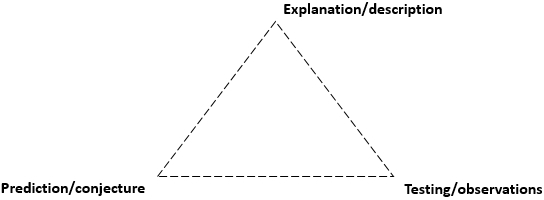
\includegraphics[scale=.5]{images/chap2-1.jpg}
\end{figure}


\section*{Defining a Problem}

The \textit{Mahābhārata} and the \textit{Rāmāyaṇa}, of their own assertion, are ‘\textit{Itihāsa}’.\index{itihasa@\textit{itihāsa}} They are ancient narratives of events of past Indian civilization. Both texts are explicit in stating their purpose, and it is easy for readers of these epics to determine for themselves, objectively, how far they succeed in their stated goals.

Pollock translates ‘\textit{Itihāsa}’ as ‘the way it once was’ (2006a:~76), as ‘accounts of the ways things were’ (2006a:~17) or as ‘an account the way things indeed were’ (2006a:~224). Nowhere is he explicit as to what he thinks of the contents of the \textit{Mahābhārata} and the \textit{Rāmāyaṇa}, as they relate to actual events of Indian history. His speculations, for the chronology\index{Chronology} of the texts of the \textit{Mahābhārata} and the \textit{Rāmāyaṇa}, focus on earliest manuscripts available and the dating of those manuscripts. Pollock\index{Pollock, Sheldon} remains, not surprisingly, oblivious to the chronology and dating of actual events described in these epics.

\newpage

\textit{Itihāsa}\index{itihasa@\textit{itihāsa}} can be meaningfully translated as ‘an ancient narrative’, ‘ancient chronicle’ or ‘traditional accounts of former events’.

Pollock’s\index{Pollock, Sheldon} speculation is restricted to identifying the timing of the first manuscript(s) of Vālmīki\index{Valmiki@Vālmīki} \textit{Rāmāyaṇa}\index{Ramayana@\textit{Rāmāyaṇa}} or Vyāsa’s\index{Vyasa@Vyāsa} \textit{Mahābhārata}. On the other hand, the actual problem to be solved is much broader than his narrow, and thus erroneous, definition for the chronology\index{Chronology} of these epics.

The problems of the \textit{Mahābhārata}\index{Mahabharata@\textit{Mahābhārata}} and the \textit{Rāmāyaṇa} chronology are as follows:

\begin{enumerate}
\itemsep=0pt
\item Is there objective evidence that would allow us to define specific lower limits (and upper limits) on the chronology of the \textit{Mahābhārata} and the \textit{Rāmāyaṇa} events?

 \item Is there objective evidence that would allow us to define specific lower limits on the chronology of the first composition of the \textit{Mahābhārata} and the \textit{Rāmāyaṇa} texts?

 \item Is there objective evidence that would allow us to define specific chronology markers (day, year or millennium) for the events of the \textit{Mahābhārata} and the \textit{Rāmāyaṇa}?

 \item Is there objective evidence that would allow us to define specific chronology markers for the first composition of the \textit{Mahābhārata} and the \textit{Rāmāyaṇa} texts and their chronological gap from the actual events of the \textit{Mahābhārata} and the \textit{Rāmāyaṇa}.

\end{enumerate}

Problem (1) is addressed in this paper. It is critical to recognize that appealing to objective evidence alone is not sufficient. This is because supporting evidence can be found for any theory if one looks for it. Testability of an evidence is what turns specific evidence into an objective evidence and it is one of the key criteria for anything to be considered as scientific evidence. Unfortunately, testability of evidence is one of the many necessary conditions of scientific investigation, but by itself, is not a sufficient condition. Confusion persists among the \textit{Mahābhārata} and the \textit{Rāmāyaṇa} researchers. Many researchers do not comprehend necessity of evaluating and testing ‘all relevant evidence’ for their theories. Ignorance of this basic premise has resulted in numerous claims for chronology of these epics that are irrational. Such claims lead to erroneous conclusions and are rather falsified easily. However, it is not easy for a lay person to recognize this problem.

A simple framework can be used to analyze any claim (not limited to chronology\index{Chronology}) related to these epics. The framework can be employed to evaluate other claims for varied aspects (when, what, why, where, how, etc.) of all ancient narratives.


\section*{Framework for Scientific Investigation of Ancient Narratives}

The following framework allows quick analysis of any claim (not limited to the \textit{Mahābhārata}\index{Mahabharata@\textit{Mahābhārata}} or the \textit{Rāmāyaṇa}\index{Ramayana@\textit{Rāmāyaṇa}}).
\begin{figure}[H]
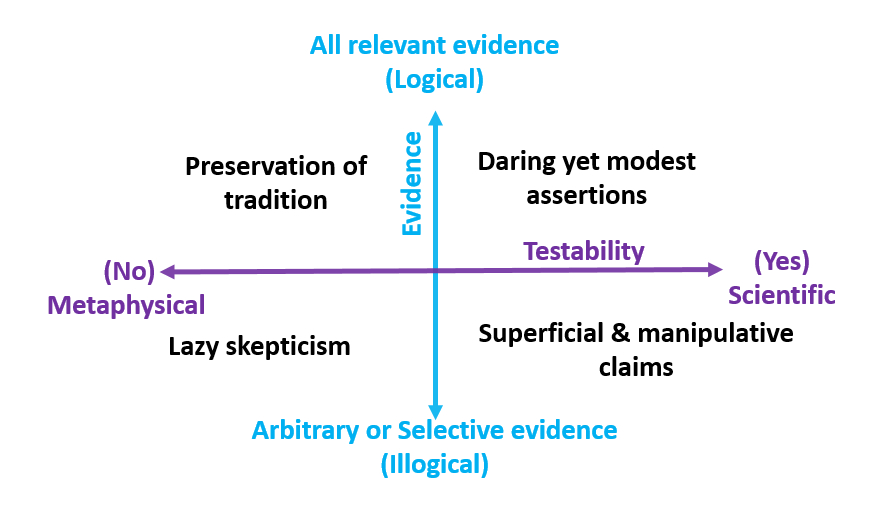
\includegraphics[scale=.3]{images/chap2-2.jpg}\\[0.2cm]
\thnum{(Figure 1)}
\end{figure}

The vertical axis of ‘evidence’ is defined by ‘all relevant evidence’ and ‘arbitrary or selective evidence’ as its endpoints. The horizontal axis of ‘testability’ is defined by discrete definitions (yes or no) as its endpoints. These simple criteria allow us to place any claim into one of the four categories (quadrants).

There are additional demands on any given claim for the consistency of a theory, corroboration and falsification outcome for each piece of relevant evidence and growth of knowledge that leads to newer problems of higher complexity. For brevity, the elaboration of these demands is not discussed in this paper.

%\newpage

A research effort that focuses on preservation of ancient narratives, without any concern for testing them to check if they are valid or not, can be described as ‘metaphysical’ and ‘rational’. This \textbf{Preservation of tradition} is a critical function, and only because of numerous individuals, our ancient heritage remains preserved for our benefit.

A research effort that focuses on analyzing all relevant evidence in the light of a specific theory and is concerned with proposing a theory in such a fashion so that all evidence becomes testable, can be described as scientific and rational. Generation of these \textbf{Daring yet modest assertions} is the desired approach.

Aware of the importanc of testability, if a research effort has a semblance of testability but otherwise lacks the rationality of including all relevant evidence, can be described as irrational and fit for scrutiny. Generation of these \textbf{Speculative and manipulative claims} is an undesirable approach. Unfortunately, a majority of research works on the dating of the \textit{Mahābhārata}\index{Mahabharata@\textit{Mahābhārata}} and the \textit{Rāmāyaṇa}\index{Ramayana@\textit{Rāmāyaṇa}} fall into this quadrant.

The remaining quadrant of \textbf{Lazy skepticism} is characterized by lack of action and metaphysical argumentation. This includes invoking of specific references/observations from the ancient narratives that are not testable (and thus metaphysical), which are then employed to argue for the futility of research efforts or to claim non-historical nature of these ancient narratives. To enable these viewpoints, the emphasis is placed on descriptions, references or observations from these epics that are non-testable. Existence of such ‘non-testable’ observations is employed to justify unauthenticity of numerous other observations that can be tested.

Metaphorically, the emphasis of research efforts and the outcome for each of these four quadrants can be described as follows (Figure 2):

A preserver of tradition will note down (and preserve) the descriptions of a flying horse with colorful wings and a crown on his head with meticulous details, free from concerns such as if the description is factually possible or not (in the real world). On the other hand, a daring yet modest asserter would search through multiple scientific disciplines and may build a theory that would be tested against available evidence for the plausible case of flying horse and may end up with only limited evidence that can corroborate existence of ‘horse like’ creature. Both approaches are ‘fearless’ and ‘humble’ in their outlook. While a preserver of tradition may invite ridicule, a daring yet modest asserter may be criticized for his inability to provide evidence in support of all the descriptions of ancient narratives. The preserver of tradition is fearless in his effort to retain and preserve all that exists in the manuscripts of ancient narratives, even when contradictions may exist within the same manuscript. The daring yet modest asserter is fearless in drawing inferences, based on testable evidence, no matter how much it conflicts with existing and established mainstream wisdom. Preserver of tradition is humble in being open about his inability to test and thus his inability to either resolve internal contradictions or verify claims of ancient narratives. Daring yet modest asserter is humble in recognizing that what can be inferred is limited by what can be tested and for this very reason acknowledging the ultimate limit in comprehension of certain descriptions of ancient narratives.

\setcounter{figure}{1}

\begin{figure}[H]
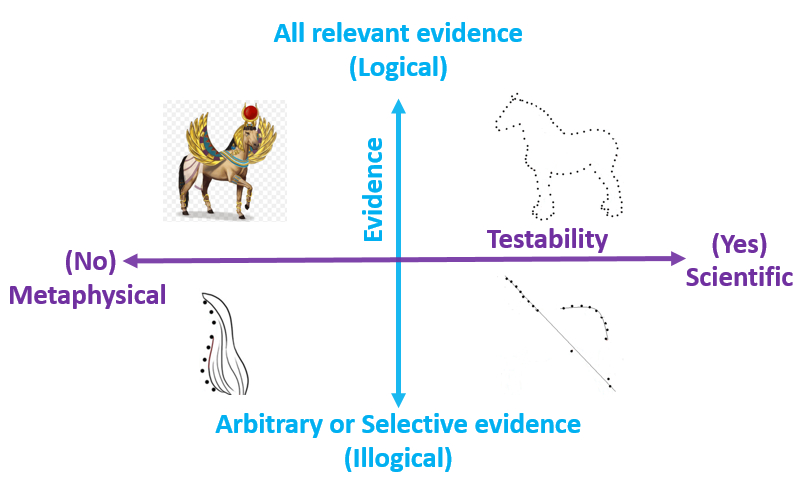
\includegraphics[scale=.3]{images/chap2-3.jpg}\\
\thnum{(Figure 2)}
\end{figure}

The efforts of the preserver of tradition leads to the preservation and availability of ancient narratives for posterity. The efforts of daring yet modest asserter, invariably, leads to the solving of the existing problem that leads to a further growth of knowledge which in turn leads to newer problems of higher complexity.

\newpage

A lazy skeptic wants to identify descriptions of ancient narratives that cannot be tested. He employs this very tactic as evidence of why researching of these ancient narratives is a futile effort. His approach not only leads to inaction on his part but may lead to inaction on the part of those who are otherwise curious to research more about ancient narratives. A lazy skeptic wants to score points via arguments and thus may ask preserver of tradition for evidence of flying horse and may ask the daring yet modest asserter for an evidence of bushy tail of the horse! For these reasons, the approach employed by the lazy skeptic is irrational and metaphysical in nature and leads to stagnation of knowledge.

A superficial manipulator invariably has \textit{a priori} answer to the problem being addressed. Not surprisingly, the approach focuses on identifying testable evidence that tends to support the answer arrived at \textit{a priori}. This results in deliberately ignoring of other testable evidence which otherwise would have falsified the preset answer. This effort should be labelled as superficial because any theory and/or proposal can always find some evidence that support the theory and/or proposal. The evidence produced is a trivially true factoid and hence superficial. On the other hand, this approach is one of a manipulator due to deliberately ignoring testable evidence that would have otherwise falsified the preset answer. This superficial manipulator is striving for quick success and want to be in a limelight and thus in a hurry to select only evidence that tends to support a specific answer while ignoring all other evidence that would falsify this preset answer. Metaphorically, this approach can be described as celebrating success based on its ability to draw a straight line or a curve through some of the data points while altogether ignoring the rest of the data points. This approach rarely, if ever, opens up newer problems of higher complexity. When done intentionally, this would amount to a fraud. When done unintentionally, it is typically due to an ignorance of scientific method, and due to a poor comprehension of the method of drawing inferences.

\vspace{-.3cm}

\section*{Development of a Theory \hfill\break and Selection of Evidence}

The development of a theory depends on the nature of problem to be solved. The selection of evidence is determined by the nature of the theory proposed. For example, validating the existence of the ancient river Sarasvatī would begin with the descriptions of the river from ancient narratives and would require a theory (or theories) that is geological, hydrological and climatological in nature and thus the corresponding evidence would also be sought from these disciplines of science. The problem of dating the \textit{Mahābhārata} or the \textit{Rāmāyaṇa}\index{Ramayana@\textit{Rāmāyaṇa}} would begin with the descriptions of testable evidence from these ancient narratives however would require a theory (or theories), for example, that are astronomical, archaeological, geological or hydrological, etc. in nature. The corresponding evidence would be sought from relevant disciplines of science, and the evidence would have to be compared against the claims/descriptions of these ancient narratives.

A claim validated by a theory based on evidence from a specific discipline (e.g. astronomy\index{Astronomy}) may luckily be validated by evidence from other disciplines (e.g. archaeology, geology, hydrology, genetics, etc.) also. In such a case, the claim might be accepted, albeit tentative, with relative ease.

While all relevant evidence is important, and must be tested for a given theory, that evidence which leads to clear restrictions on the plausible choices (When? Where? What? How? etc.) is the most prized evidence. Such prized evidence conduces to a sound growth of knowledge. In other words, a scientific investigation that eliminates certain choices as plausible options is much more valuable than the one that tends to provide support for an existing proposition.

\vspace{-.3cm}

\section*{Astronomy-theory and Evidence \textit{vis-à-vis} \hfill\break the \textit{Mahābhārata}\index{Mahabharata@\textit{Mahābhārata}} and the \textit{Rāmāyaṇa}}

Astronomical data includes descriptions of star positions, descriptions of planets – their positions, their specific motions and their conjunctions with other planets and/or \textit{nakṣatra},\index{naksatra@\textit{nakṣatra}} descriptions of comets, solar and lunar eclipses, positions and phases of the moon, descriptions of the seasons, descriptions of nature during specific lunar months and lunar \textit{tithi}.\index{tithi@\textit{tithi}} Numerous chronological narrations, when coupled with astronomy markers such as seasons or cardinal points of solstices and equinoxes, also constitute astronomical evidence.

The \textit{Mahābhārata} text has more than 200 astronomy and chronology\index{Chronology} observations and testing of them leads to 5561 BCE as the year of \textit{Mahābhārata} war\index{Bharata war@Bhārata war}. The Vālmīki \textit{Rāmāyaṇa} text has more than 500 astronomy\index{Astronomy} and chronology observations and testing of them leads to 12240 BCE as the year of the birth of Rāma, and 12209 BCE as the year of Rāma-Rāvaṇa\index{Rama-Ravana yuddha@Rāma-Rāvaṇa \textit{yuddha}} \textit{yuddha}.

Testing of two astronomical observations, one each from the \textit{Mahābhārata} text and the Vālmīki\index{Valmiki@Vālmīki} \textit{Rāmāyaṇa} text, out of a total of ~800 relevant observations from these two epics, is demonstrated which in turn lead to lower limits of 4500 BCE and 10,000 BCE, on the chronology\index{Chronology} of the \textit{Mahābhārata}\index{Mahabharata@\textit{Mahābhārata}} and the \textit{Rāmāyaṇa},\index{Ramayana@\textit{Rāmāyaṇa}} respectively.

A comprehension of the astronomical phenomenon of the precession\index{Precession of Equinoxes} of equinoxes (explained later) and its resulting consequences is a prerequisite to understand the testing of these two astronomical observations, and their implications for the chronology of the \textit{Mahābhārata} and the \textit{Rāmāyaṇa}.

\vspace{-.3cm}

\section*{Precession of Equinoxes}

The Precession of equinoxes is the phenomenon of the movement of the earth's axis in a circular path that takes about 26000 years to complete one cycle. As the earth’s axis moves through a circular path, it traces a circle in the sky. At any given time, where the earth's axis points to, along this circular path, is called the point of the North Celestial Pole (\textbf{NCP}). If a distinct and visible star is close to this point of NCP, it attains the status of a North Pole\index{North Pole star} Star (\textbf{NPS}) the period, i.e. until the NCP moves far away from the position of the star.

\textbf{This results in:}

\begin{enumerate}
\itemsep=0pt
\item 
 Change in the location of NCP and thus also the change of NPS.

 For example, while ‘Polaris’\index{Polaris} is NPS in our times, Vega (Abhijit\index{Abhijit}/Brahmarāśi\index{Brahmarasi@Brahmarāśi}) was the NPS around 12000 BCE (Figure 3).

 \item Change in the position of the Sun (with respect to the reference frame of the background \textit{nakṣatra})\index{naksatra@\textit{nakṣatra}} for specific cardinal points.

 For example, timing (day, Lunar month and \textit{tithi})\index{tithi@\textit{tithi}} of Winter Solstice\index{Winter Solstice} would shift with respect to the background reference frame of the \textit{nakṣatra}, by about one day (one degree) every 72 years. This means the point of Winter Solstice would shift by about one \textit{nakṣatra} every (26000/27 = 963 or approximately a 1000) thousand years.

 In the present context (2016 CE), the position of the Sun is between \textit{nakṣatra}\index{naksatra@\textit{nakṣatra}} Mūlā\index{Mula@Mūlā} and \textit{nakṣatra} Pūrva Āṣāḍha\index{Purva Asadha@Pūrva Āṣāḍha} on the day of Winter Solstice\index{Winter Solstice}, and is between \textit{nakṣatra} Ārdrā\index{Ardra@Ārdrā} and \textit{nakṣatra} Mṛgaśīrṣa\index{Mrgasirsa@Mṛgaśīrṣa} on the day of Summer Solstice\index{Summer Solstice} (Figure 4).


\begin{figure}[!h]
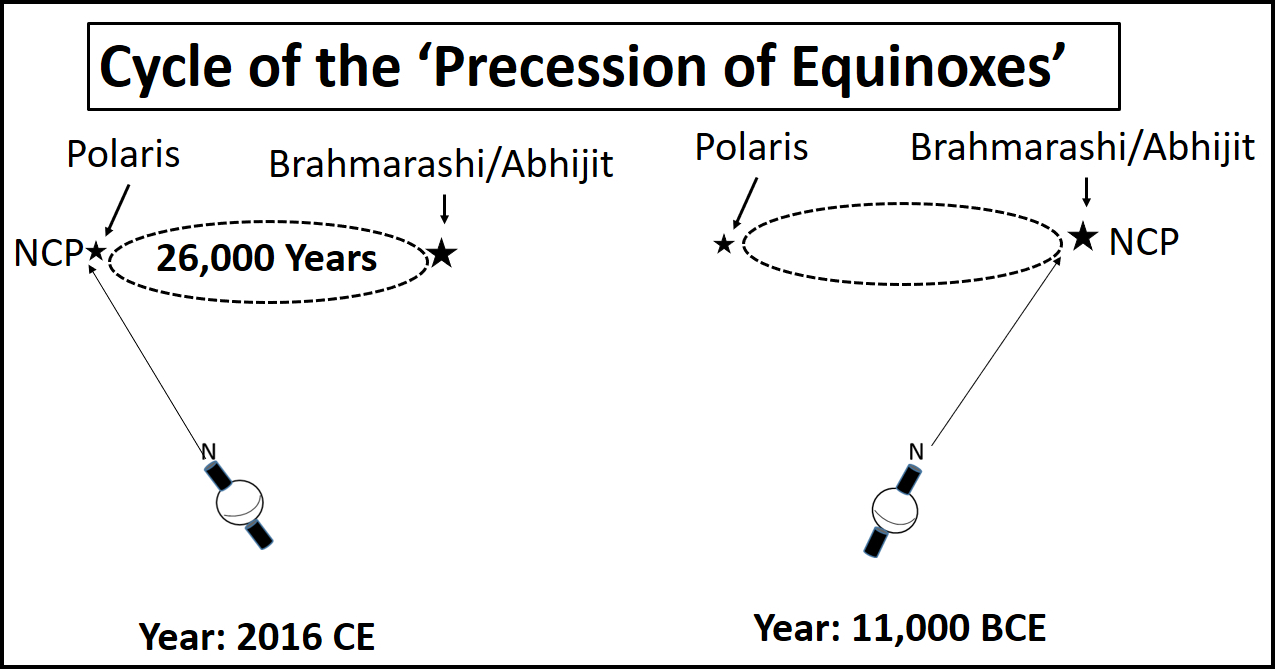
\includegraphics[scale=.17]{images/chap2-4.jpg}\\[0.1cm]
\thnum{(Figure 3)}
\end{figure}


\begin{figure}[!h]
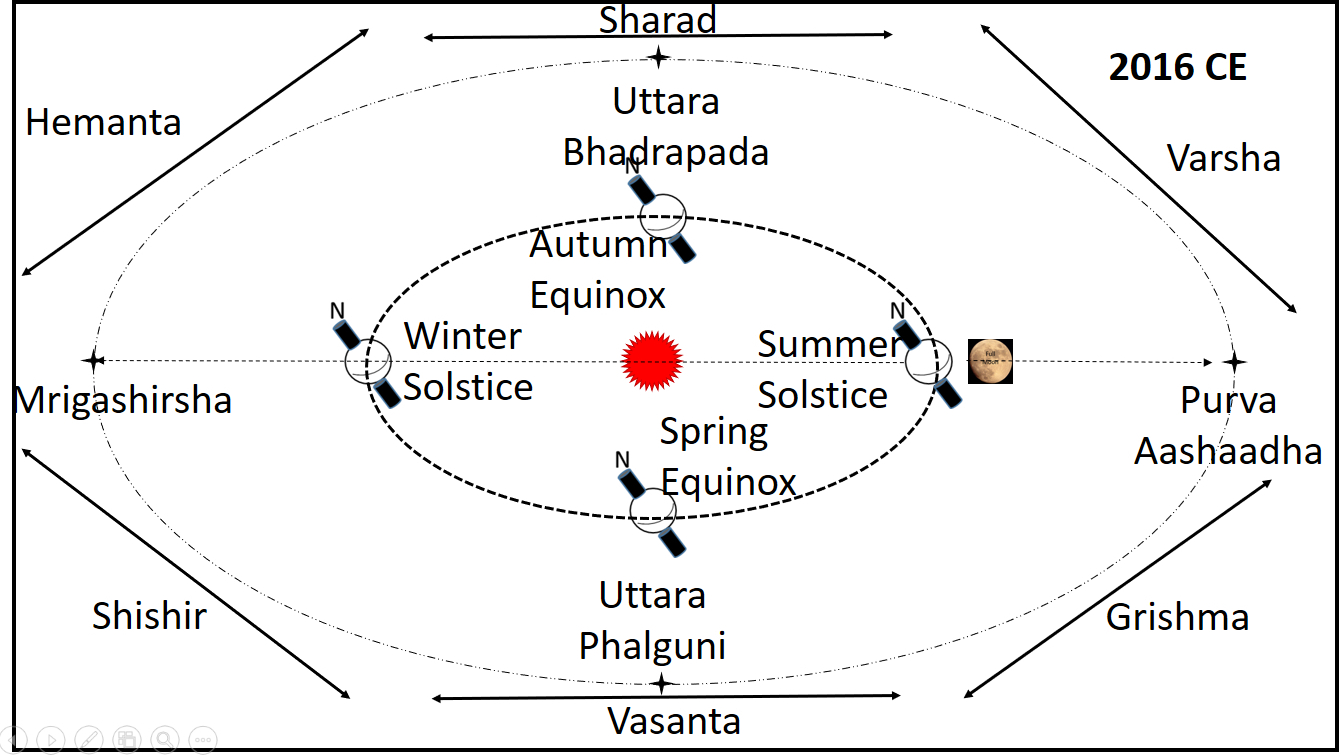
\includegraphics[scale=.165]{images/chap2-5.jpg}\\[0.1cm]
\thnum{(Figure 4)}
\end{figure}

If we go back in antiquity by about 7500 years, the position of the sun for the day of Winter Solstice, would shift from \textit{nakṣatra} Mūlā/Pūrva Āṣāḍha to \textit{nakṣatra} Uttara Bhādrapada; and the position of the Sun for the day of Summer Solstice, would shift from \textit{nakṣatra} Ārdrā/Mṛgaśīrṣa to \textit{nakṣatra} Hastā\index{Hasta@Hastā}/Uttara Phalgunī. A shift of about 7 \textit{nakṣatra}-s would occur, as expected, corresponding to ~7000 years. (Figure 5)


\begin{figure}[!h]
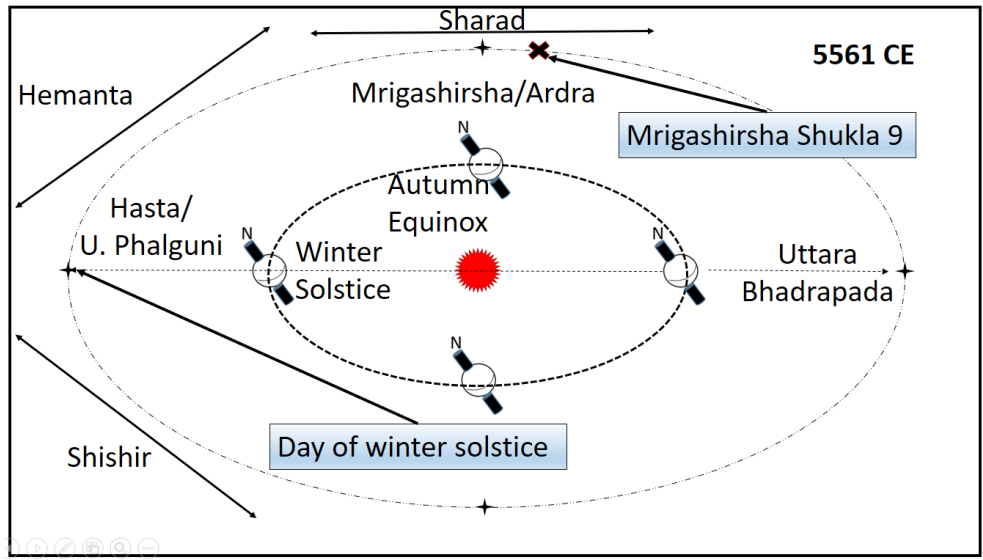
\includegraphics[scale=.2]{images/chap2-6.jpg}\\[0.1cm]
\thnum{(Figure 5)}
\end{figure}

\newpage


 \item 
 Change (shift) of season with respect to calendar, by about one lunar month every 2000 years.


\begin{figure}[!h]
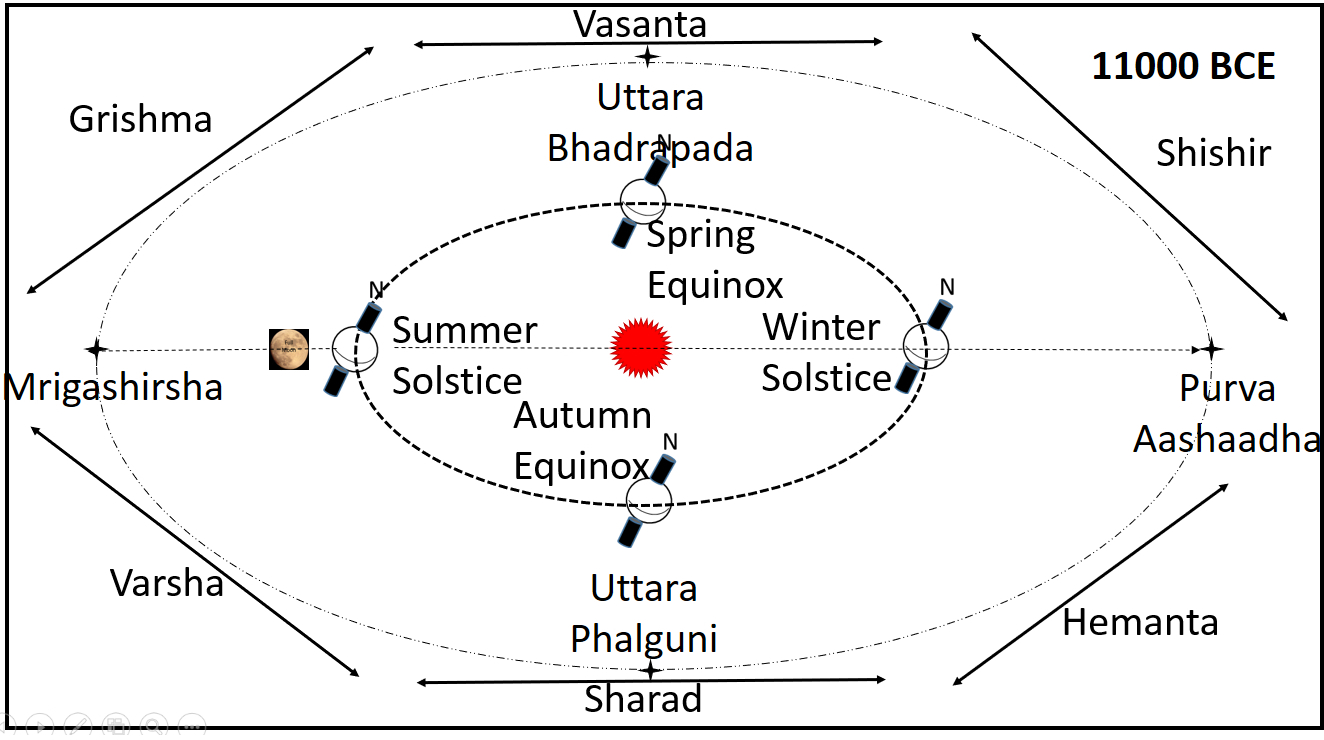
\includegraphics[scale=.16]{images/chap2-7.jpg}\\[0.1cm]
\thnum{(Figure 6)}
\end{figure}

Lunar month of Caitra occurs during the second half of Vasanta \textit{ṛtu} (Spring) in our times. If we go back, halfway through the cycle of the precession\index{Precession of Equinoxes} of equinoxes, to ~11000 BCE, lunar month of Caitra coincided with the second half of Śarad \textit{ṛtu} (pre-autumn). Lunar month of Āśvina occurs during the second half of Śarad \textit{ṛtu} (pre-autumn) in our times. If we go back halfway through the cycle of the precession of equinoxes, to ~11,000 BCE, lunar month of Āśvina coincided with the second half of Vasanta \textit{ṛtu} (spring). In other words, the points of all cardinal points (solstices and equinoxes) had reversed (2016 CE vs 11000 BCE) (Figure 4 vs Figure 6).

\end{enumerate}


\section*{An Illustration from the \textit{Mahābhārata} text}

Vyāsa\index{Vyasa@Vyāsa} met Dhṛtarāṣṭra\index{Dhrtarastra@Dhṛtarāṣṭra} on the day before the first day of \textit{Mahābhārata} war\index{Bharata war@Bhārata war}, as a final attempt, to avoid the war. Vyāsa mentioned series of omens (\textit{nimitta}) to Dhṛtarāṣṭra and among them was this peculiar one:

\vspace{0.15cm} 

\textbf{Bhīṣma Parvan} (2.31) (Gita Press and Critical Edition)
\begin{verse}
\textit{yā caiṣā viśrutā rājaṁstrailokye sādhusaṁmatā \dev{।}}\\
\textit{arundhatī tayāpyeṣa vasiṣṭhaḥ pṛṣṭhataḥ kṛtaḥ \dev{॥}}
\end{verse}

\vspace{-.3cm}

\vspace{0.1cm} 

(Gist: Renowned and well respected Arundhatī has gone ahead of Vasiṣṭha)

\vspace{0.15cm} 

Majority of the \textit{Mahābhārata}\index{Mahabharata@\textit{Mahābhārata}} researchers were too perplexed by this astronomy\index{Astronomy} observation to even dare mention it in their analysis. Few researchers mentioned Arundhatī\index{Arundhati@Arundhatī}\index{Arundhati-Vasistha@Arundhatī-Vasiṣṭha}-Vasiṣṭha\index{Vasistha@Vasiṣṭha} (AV) observation only to explain it away. Bharata Ratna and Mahāmahopādhyāya Pandurag Vaman Kane\index{Kane, P. V.} wrote, referring to AV observation:

\vspace{0.15cm} 

\begin{myquote}
The author or authors of the \textit{Mahābhārata}, in describing the evil portents of an impending tragic or catastrophic event, often assemble such observations \textbf{irrespective of the fact whether some of them are possible in the very order of nature}. 

\vspace{0.1cm} 

~\hfill (Kane 1968: 905) \textit{(emphasis ours)}
\end{myquote}

\vspace{0.15cm} 

Bharatāchārya C. V. Vaidya (1905:~84) compared his shock at the description of AV observation with that of biologically implausible absurdities:

\vspace{0.15cm} 

\begin{myquote}
The last editor probably wished to accumulate the number of the evil omens which preceded the war and tried to put in such impossible combinations as he could bring together. \textbf{For instance,… the statement that Arundhati went before Vasishtha among the Saptarishis.} These may be classed with absurdities in the animal world mentioned further on such as the birth of a cow from a mare or a jackal from a dog. 

\vspace{0.1cm} 

~\hfill (Vaidya 1905: 83-84) \textit{(emphasis ours)(spelling as in the original)}
\end{myquote}

\vspace{0.15cm} 


Professor R. N. Iyengar (2006) began with AV observation reference, but only partially, and combined it with another non-relevant and partial reference from another chapter of Bhīṣma Parvan, presumably to make some sense out of this AV observation, on which Prof. Iyengar’s article does not shed much light.

More than half of the over 130 \textit{Mahābhārata} researchers have employed astronomy\index{Astronomy} evidence as their basis in proposing those many different dates for the chronology\index{Chronology} of the \textit{Mahābhārata} war\index{Bharata war@Bhārata war} and none of them, apart from Dr. P. V. Vartak, dared to analyze AV observation. These researchers avoided AV observation as if it was a poison pill\index{poison pills}. This is especially intriguing when it can be shown that these same researchers refer to three of the four astronomy observations from the same chapter of Bhīṣma Parvan, fourth observation being that of Arundhatī\index{Arundhati@Arundhatī}-Vasiṣṭha\index{Arundhati-Vasistha@Arundhatī-Vasiṣṭha}\index{Vasistha@Vasiṣṭha}. Even more perplexing is the fact that AV observation appears very much in the middle of these astronomy observations.

What can explain the aversion and reluctance of these \textit{Mahābhārata}\index{Mahabharata@\textit{Mahābhārata}} researchers to this AV observation ‘poison pill’? It is not difficult to understand their dilemma. They were at loss to explain or to test this observation. This is because Arundhatī-Vasiṣṭha form a stable star-pair and Vasiṣṭha is walking ahead of (moving ahead of) Arundhati, in an anticlockwise direction, around Polaris\index{Polaris} - the north pole star\index{North Pole star}, in our times. In addition, even if we simulate movement of Arundhatī and Vasiṣṭha, further back by 2000, 4000 or 6000 years, in antiquity, Vasiṣṭha would have still appeared walking ahead of Arundhati. On the other hand, many of these researchers had assumed, without much basis and a priori, that the \textit{Mahābhārata} war had occurred, within last ~5000 years.

Only one the \textit{Mahābhārata} researchers, Dr. P. V. Vartak, was convinced of the factual nature of AV observation. Dr. Vartak made various attempts to test this observation empirically however failed. This author became aware of AV observation sometime in 1995 CE and thought, naively, that it would be easy to test and validate this observation empirically. Fifteen years of uninterrupted efforts led to empirical validation of this observation on 8 May 2009 CE.

Relative positions of Arundhatī (Alcor) and Vasiṣṭha (Mizar) with respect to the north pole star (Polaris) are shown in Figure 7.

\begin{figure}[H]
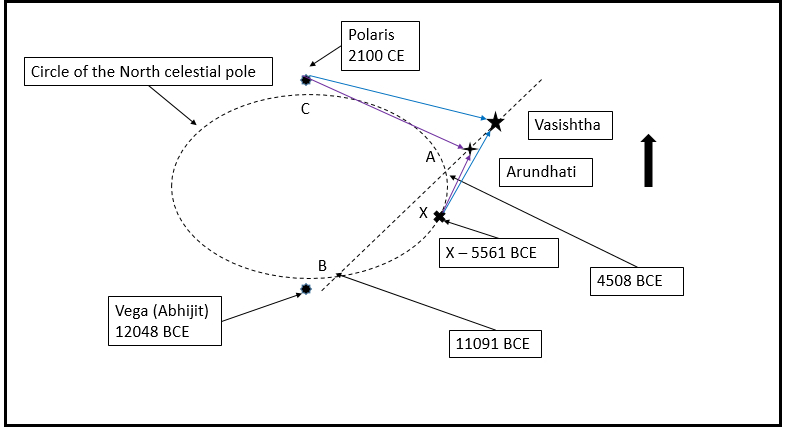
\includegraphics[scale=.3]{images/chap2-8.jpg}\\[0.1cm]
\thnum{(Figure 7)}
\end{figure}

\begin{enumerate}
\itemsep=0pt
\item Arundhatī\index{Arundhati@Arundhatī} and Vasiṣṭha\index{Arundhati-Vasistha@Arundhatī-Vasiṣṭha}\index{Vasistha@Vasiṣṭha} go around Polaris\index{Polaris} (point C), not unlike two end points of the long and short arms of a wall clock, except in anticlockwise direction, and complete one round in 24 hours. Their relative positions are such that Vasiṣṭha would appear to walk ahead of Arundhatī. The dotted line circle represents the path of north celestial pole (NCP) also known as the precession of equinoxes\index{Precession of Equinoxes} that completes one round in about 26000 years. If a straight line is drawn through Arundhatī and Vasiṣṭha, it intersects the circle of NCP at two points (A and B). These two points correspond to positions of NCP in year 4508 BCE and 11091 BCE, respectively.

 \item When points of NCP are at A or B, Arundhatī and Vasiṣṭha would appear to walk around these points of NCP, again anticlockwise, with no one ahead and no one behind.

 \item The third scenario occurs when the point of NCP is anywhere along the path of the NCP designated by portion of the circle AXB. As shown by the point X, which represents the position of NCP in the year 5561 BCE, Arundhatī and Vasiṣṭha would walk around this point X, again anticlockwise, but this time Arundhatī would appear to walk ahead of Vasiṣṭha.

\end{enumerate}

There was, thus, indeed a time interval, in antiquity, beginning with 11091 BCE and ending with 4508 BCE, when Arundhati indeed appeared to walk ahead of Vasiṣṭha. This time interval (Epoch of Arundhati) defines the boundaries where one should search for the year of the \textit{Mahābhārata} war. Keeping aside the question of the exact year of the \textit{Mahābhārata} war, what can be said with mathematical certainty is that the \textit{Mahābhārata} war did not take place any time after 4508 BCE. AV observation and its validation presented an excellent illustration of \textit{śabda pramāṇa}\index{sabda@\textit{śabda}} validated by \textit{pratyakṣa pramāṇa}\index{pratyaksa@\textit{pratyakṣa}} that also puts a strict lower limit of 4508 BCE (poison pill\index{poison pills}) on the chronology\index{Chronology} of the \textit{Mahābhārata}.

The revolutionary outcome of AV observation can be understood in the context of the triad of explanation-testing-prediction. While the description of AV observation was unambiguous, no prior researcher had succeeded in testing it empirically. However as soon as the empirical test validated the description, it led to a clearly marked time interval for the year of the \textit{Mahābhārata} war\index{Bharata war@Bhārata war}. In this case, the prediction of the time interval for the year of the \textit{Mahābhārata}\index{Mahabharata@\textit{Mahābhārata}} war was the invaluable insight!

\begin{figure}[!h]
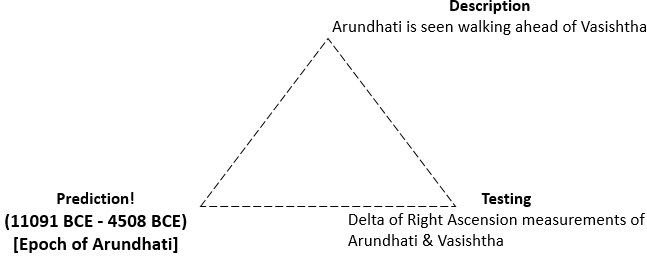
\includegraphics[scale=.38]{images/chap2-9.jpg}
\end{figure}

The validation of AV observation was only the beginning of a long journey as more than 200+ additional astronomy\index{Astronomy}, chronology and seasonal observations existed, and their meticulous testing led to 5561 BCE as the year of the \textit{Mahābhārata} war and 16 October 5561 BCE (Julian calendar computation) as the first day of the \textit{Mahābhārata} war.

\vspace{-.3cm}

\section*{An Illustration from \hfill\break the Vālmīki\index{Valmiki@Vālmīki} \textit{Rāmāyaṇa}\index{Ramayana@\textit{Rāmāyaṇa}} text }

The Vānara search party returned to Kiṣkindhā with news of Sītā. Rāma and Lakṣmaṇa, along with Sugrīva and his Vānara army, marched towards Laṅkā. It is during this time, Lakṣmaṇa mentioned numerous omens and among this list, he described the north pole star\index{North Pole star} of the \textit{Rāmāyaṇa} times:

\newpage

\textbf{Yuddha Kāṇḍa}\index{Yuddhakanda@Yuddha Kāṇḍa} (Gita Press Edition 4:48, Critical Edition 4:43)

\begin{verse}
\textit{brahmarāśir viśuddhaś ca śuddhāś ca paramarṣayaḥ \dev{।}}\\\textit{arciṣmantaḥ prakāśante dhruvaṁ sarve pradakṣiṇam \dev{॥}}
\end{verse}

\textbf{(Gist: Seven pure sages are making \textit{parikrama} around fixed Brahmarāśi,\index{Brahmarasi@Brahmarāśi} the pole star)}

The position of the north celestial pole (NCP) slowly moves in a circular path and completes one cycle in about 26000 years (Figure 3). If a bright star happens to be next to the point of NCP, it attains the status of a north pole\index{North Pole star} star, for some time. Polaris\index{Polaris} is the north pole star in our times and will attain a position closest to the point of NCP around 2100 CE. If we simulate the skies for the point of NCP,

Kochab was the north pole star around 2100 BCE,

Thuban around 2800 BCE, Brahmarāśi (also known as Abhijit\index{Abhijit} or Vega) around 12000 BCE and Deneb around 16000 BCE (Figure 8).

\begin{figure}[!h]
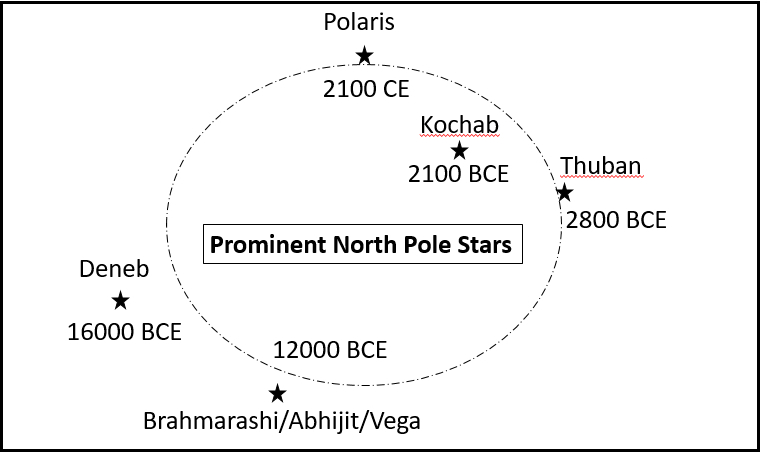
\includegraphics[scale=.32]{images/chap2-10.jpg}\\[0.1cm]
\thnum{(Figure 8)}
\end{figure}

Vālmīki\index{Valmiki@Vālmīki} \textit{Rāmāyaṇa}\index{Ramayana@\textit{Rāmāyaṇa}} refers to ‘Brahmarāśi’ as the north pole star. Brahmarāśi would have attained and retained a status as north pole star for about ±1000 or 2000 years around 12000 BCE, when the point of NCP was closest to Brahmarāśi. Star Vega is mentioned multiple times as Abhijit and Brahmarāśi (\textit{Rāmāyaṇa}) or Brahmarāśi, \textit{nakṣatra}\index{naksatra@\textit{nakṣatra}} of Brahma and Abhijit (\textit{Mahābhārata})\index{Mahabharata@\textit{Mahābhārata}} in these epics. The validation of Brahmarāśi as the north pole star of \textit{Rāmāyaṇa} times defines the interval of 10000 BCE – 14000 BCE where one should search for the plausible chronology\index{Chronology} of \textit{Rāmāyaṇa}. And keeping aside the question of the exact year of the birth of Rāma or the battle between Rāma and Rāvaṇa, it can be stated with mathematical certainty that the \textit{Rāmāyaṇa} did not take place any time after 10000 BCE.

The revolutionary outcome of the Brahmarāśi\index{Brahmarasi@Brahmarāśi} observation can be understood in the context of the triad of testing-prediction-explanation by recognizing that while the identification of various stars for their status as north pole\index{North Pole star} stars was well known, and the timing when they attained such status could be easily tested, no prior researcher had comprehended either the value of Brahmarāśi observation for the dating of the \textit{Rāmāyaṇa},\index{Ramayana@\textit{Rāmāyaṇa}} and/or identification of Brahmarāśi with that of Abhijit/Vega. However as soon as these two insights dawned upon, it led to a clearly marked time interval for the year of Rāma-Rāvaṇa\index{Rama-Ravana yuddha@Rāma-Rāvaṇa \textit{yuddha}} battle and hence of the \textit{Rāmāyaṇa}. In this case, the recognition of Brahmarāśi observation and identification of Brahmarāśi with that of Abhijit\index{Abhijit}/Vega – were the two invaluable insights!

\begin{figure}[!h]
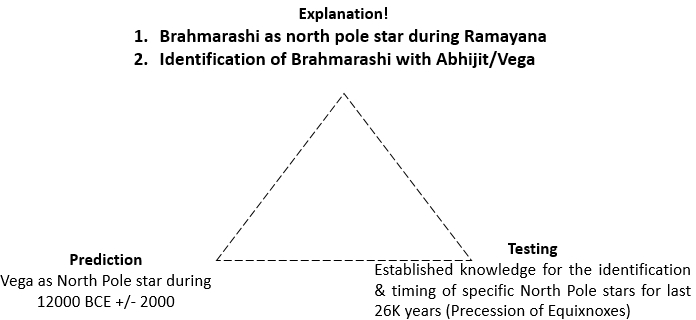
\includegraphics[scale=.4]{images/chap2-11.jpg}
\end{figure}

The testing of Brahmarāśi observation defined a time interval for the plausible timing of the \textit{Rāmāyaṇa}. This was only the beginning of a long journey as more than 500+ additional observations pertaining to astronomy\index{Astronomy}, chronology and seasons, and their meticulous testing led to 12209 BCE as the year of Rāma-Rāvaṇa battle, and 12240 BCE (Julian calendar computations) as the year of Rāma-janma.


\section*{Way Forward}

Preservers of tradition are doing their jobs and daring yet modest asserters are proposing bold theories and then testing them against the available evidence, to develop/improve our knowledge of ancient Indian civilization. Manipulators with superficial knowledge put forward numerous proposals do not stand scrutiny. The refutation of such numerous \textit{ad hoc} proposals also leads to a growth of knowledge – by eliminating the impossible.

Researches of Videshi Indology may fall, occasionally, into ‘lazy skeptics’ quadrant, however, for most part they do not follow either evidence based or logic based thought process. Therefore, efforts of swadeshi Indology should be limited to demonstrating illogical and unscientific nature of Videshi Indology works. On the other hand, swadeshi Indology researchers should concentrate their efforts on producing new research that is logical and evidence based.


\section*{Poison Pills\index{poison pills}}

Discovery of these two pieces of evidence, their empirical testing and their implications for the chronology of the \textit{Mahābhārata}\index{Mahabharata@\textit{Mahābhārata}} and the \textit{Rāmāyaṇa}\index{Ramayana@\textit{Rāmāyaṇa}} were made less than ten years ago and will serve as ‘poison pills’ against any dogmatic and extreme views for the chronology\index{Chronology} of these epics. Even those who do comprehend the revolutionary impact of this evidence express concern. They worry that opposing and dogmatic forces might raise an objection such as “but these are only two references and it could be just a coincidence that their testing led to prediction of a time interval with crisp lower bounds”. Such objections are not based on facts. We should eagerly encourage not only Videshi Indologists and but also researchers of existing dogmatic claims to study and challenge these claims. While these two observations and their implications have produced ‘poison pills’ par excellence, this is only the beginning. More than 800 astronomy\index{Astronomy} and chronology observations from these two epics have generated numerous additional poison pills, e.g., empirical testing of set of astronomy and chronology references related to Bhīṣma-Nirvāṇa, from the \textit{Mahābhārata} text, also leads to 4500 BCE as the lower limit on the chronology of the \textit{Mahābhārata} war\index{Bharata war@Bhārata war}; and empirical testing of three additional observations from three different sections (\textit{kāṇḍa}) of Vālmīki\index{Valmiki@Vālmīki} \textit{Rāmāyaṇa} independently corroborate lower limit of 10000 BCE established by Brahmarāśi\index{Brahmarasi@Brahmarāśi} observation.

Additional evidence is pouring in, from varied disciplines of science – geology, anthropology, paleontology, astronomy\index{Astronomy}, genetics, hydrology, oceanography, seismology and climatology that provide strong corroborative support for these chronology\index{Chronology} claims.

Pollock\index{Pollock, Sheldon} comments in assigning very recent timeline for the composition of these epics:

\begin{myquote}
Only an ideology of antiquity and the cultural distinction conferred by sheer age have induced scholars to move them back appreciably before this date—a move that requires conjecture every step of the way and the most fragile gossamer of relative dating. 

~\hfill (Pollock 2006a: 81)
\end{myquote}

This very statement of Pollock ought to be modified in the context of accumulating evidence for the deep antiquity of these epics and that apply, fittingly, to irrational and metaphysical approach of Pollock:

\textit{Only an ideology of Hinduphobia\index{Hinduphobia} and the smugness conferred by sheer time spent in Indology has induced Pollock to move them forward to a date at the beginning of a common era – a move that requires citing negative evidence every step of the way and the most fragile gossamer of relative dating.}


\section*{The Epics as Unitary Works}

Pollock writes in his introduction to the translation of ‘Araṇya Kāṇḍa\index{Aranya Kanda@Araṇya Kāṇḍa}’ in the Clay series:

\begin{myquote}
The problem of what unifies these two very different sections of the poem [referring to Ayodhyā\index{Ayodhya Kanda@Ayodhyā Kāṇḍa} and Araṇya Kāṇḍa sections of Vālmīki \textit{Rāmāyaṇa}\index{Ramayana@\textit{Rāmāyaṇa}}] remains a challenging one. In the case of ‘The Ramáyana’ the view persists that the poem is a fusion or amalgamation of two very different and in fact unrelated stories. Not only has the need to develop a unitary understanding of the poem been eliminated by eliminating the perception of the poem as a unitary work, but what in this tradition has been considered the first and greatest poem, and venerated as such for two thousand years, is now declared to be, not a meaningful whole – as Indian audiences have invariably taken it to be – but a congeries of utterly distinct and unrelated materials. 

~\hfill (Pollock 2006b: 15-16)
\end{myquote}

The cumulative evidence of 800+ testable observations from the \textit{Mahābhārata} and the \textit{Rāmāyaṇa}\index{Ramayana@\textit{Rāmāyaṇa}} text, establishes beyond doubt, whether one is talking of either eighteen \textit{parvan}-s of \textit{Mahābhārata}\index{Mahabharata@\textit{Mahābhārata}} or seven \textit{kāṇḍa}-s of the \textit{Rāmāyaṇa}, that they form a unified whole. However, elaboration of this assertion would require a longer discussion, which is beyond the purview of this paper.


\section*{Bibliography}

\begin{thebibliography}{99}
\itemsep=1pt
\bibitem{chap2-key01} Iyengar, R. N. (2003). “Internal Consistency of Eclipses and Planetary Positions in \textit{Mahābhārata}”. \textit{Indian Journal of History of Science}, 38.2 (2003). pp. 77--115.

 \bibitem{chap2-key02} Bhatt, G. H. (1958). \textit{The Vālmīki Rāmāyaṇa (Critical Edition).} Baroda: Oriental Institute.

 \bibitem{chap2-key03} Kane, Pandurang Vaman. (1968). \textit{History of Dharmaśāstra} Volume III. Pune: Bhandarkar Oriental Research Institute.

 \bibitem{chap2-key04} Oak, Nilesh. (2011). \textit{When did the Mahābhārata war Happen?: The Mystery of Arundhati}. Danphe Inc., USA.

 \bibitem{chap2-key05} —. (2014). \textit{The Historic Rama: The Indian civilization at the end of Pleistocene}. CreateSpace Independent Publishing, USA.

 \bibitem{chap2-key06} Pollock, Sheldon. (2006a). \textit{The Language of the Gods in the World of Men.} Berkley: University of California Press.

 \bibitem{chap2-key07} —. (2006b). \textit{Rāmāyaṇa} \textit{Book Three: The Forest by Vālmīki.} New York: New York University Press and JJC Foundation.

 \bibitem{chap2-key08} \textit{Mahābhārata, The.} (1971). Critical Edition. Pune: Bhandarkar Oriental Research Institute.

 \bibitem{chap2-key09} \textit{Mahābhārata, The.} (1955). Gita press edition with Sanskrit text and Hindi translation. Gorakhpur: Gita Press.

 \bibitem{chap2-key10} \textbf{\textit{Mahābhārata, The.}} (Southern Recension). See Sastri (1931).

 \bibitem{chap2-key11} \textit{Rāmāyaṇa} of Vālmīki (2006). Gita Press Edition with Sanskrit text and English translation Gorakhpur: Gita Press.

 \bibitem{chap2-key12} \textbf{\textit{Rāmāyaṇa}} of Vālmīki. See Bhatt (1958).

 \bibitem{chap2-key13} Sastri, P. P. S. (Ed.) (1934). \textit{The Mahābhārata (Southern Recension).} (Critically Edited). Madras: Ramaswamy Sastrulu \& Sons.

 \bibitem{chap2-key14} Vaidya, C. V. (1905). \textit{The Mahābhārata: A Criticism.} Bombay: A. J. Combridge \& Co.

 \bibitem{chap2-key15} Vartak, Padmakar. (2012). \textit{Swayambhu}. Pune: Ved Vidnyana Mandal.

 \end{thebibliography}

\label{chapter2-end}
